\section{Source audit and controlled measurements}
\label{sec:experiments}

The experiments support two different conclusions. The new operation gives
a substantial checked group-stage improvement on the explicit source family
of Section~\ref{sec:family}. It does not improve the total running time of the
preserved ordinary corpus. We retain both findings, the unsuccessful eager
policy, and every recorded bounded nondecision. The proofs establish the
asymptotic statements; finite timing measurements test the implementation
and the mechanism responsible for its observed behavior.

\subsection{Independent package isolation and timing boundary}

The comparison imports the complete Python package from the pinned commit
and the complete modified package in separate persistent worker processes.
Both are imported under their normal name, \code{fastunknot}. This matters
because some maintained modules use absolute imports: loading two versions
under aliases inside one Python process can accidentally mix their
dependencies and invalidate a comparison. Frozen package trees are included
in the archive. Every Python source file, and the measurement harness itself,
is hashed before and after a run. Those hashes are identical across the
final guarded audit and both timing experiments.

The worker measures exactly
\begin{lstlisting}[language=Python]
start = time.perf_counter()
result = fn(Diagram.from_pd(pd), **options)
elapsed = time.perf_counter() - start
\end{lstlisting}
where \code{fn} is \code{group_decide} for the stage experiment and
\code{recognize} for the ordinary corpus. The interval includes fresh source
validation and the complete call, including mandatory independent compressed
source replay whenever a group certificate is produced. Package import,
transport between processes, traversal of
the returned evidence, and JSON serialization are outside the interval.
The timing is therefore a completed checked call, not just a favorable
inner kernel.

Each input has six arms: predecessor default, predecessor forest, delivered
singleton, and an identical A/A repeat of each. Each arm has one excluded
warmup. Five subsequent rounds are retained; the six arms are randomly
shuffled within each round using a fixed recorded seed. The workers use
\code{PYTHONHASHSEED=0}. The environment was Python 3.12.14 on
Linux 6.18.44, x86-64, glibc 2.39. The precise inputs, options, sample orders,
statuses, counters, proof objects, and hashes are in the result JSON files.

Tables report the median elapsed time of each named arm. A displayed
comparison ratio is the median of the five within-round time ratios;
it is not the ratio of the two displayed medians. A ratio above one favors
the singleton arm. A/A controls reveal ordinary timing variation, especially
on submillisecond cases. This is a single-environment experiment with five
measured rounds, not a statistical confidence interval or evidence of a
universal wall-time improvement.

\subsection{Source-bound audit and regression coverage}

The guarded audit contains 81 validated source cases, comprising 75 distinct
planar-diagram arrays: the preserved
19-case corpus, fixed-seed valid one-component braid closures, and seven
stabilized circles. For each source, it compares the predecessor and current
implementation with all new options disabled, with primitive projection,
and with primitive forest. All 243 comparisons agree exactly in the returned
certificates or bounded nondecisions. Their recorded statistics also agree.
This comparison uses the whole pinned package and checks compatibility
of the existing modes, rather than comparing against a reimplemented model.

With the singleton option enabled, 54 sources yield positive certificates.
All 54 pass both the literal and the compressed independent source replayers.
There are no newly closed and no lost positive cases relative to either
predecessor default or predecessor forest in this finite audit. Of the 54
proofs, 29 use version eight, 22 use version five, and three use version one.
The version-eight proofs contain 29 batches and 307 certified pivots.
An unsuccessful attempt is not counted as a successful certified batch.

The maintained test suite discovers and runs 1,008 tests successfully, with
zero failures, errors, or skips. This is the pinned suite plus 16 new test
methods. The authoritative ledger records the completed count, source hashes,
Python version, and empty failure and error lists. Historical reference
modules imported by older tests are included with the reproduction snapshot.

The new methods contain 80 randomized metadata cases and 100 randomized
signed DAG cases, including orders that disagree with numeric label order.
They compare every retained relator with literal substitution, test actual
stabilized diagrams through 128 crossings, exercise huge shared powers and
the $2^{511}$ raw-length family, and check resource exhaustion and caller
cancellation. Adversarial cases include duplicate slots, duplicate pivots,
boolean identifiers, fabricated singleton conditions, dependency cycles,
old-version relabelling, and an obstructing residual relation that must be retained.
Selected tests disable producer helpers, normalization, or expansion during
compressed replay to check the intended independence and raw boundary.

A separate small exhaustive review enumerates 3,698 ordered local cases over
three generators. Exactly 360 are accepted and 3,338 rejected, with exact
agreement between the independently computed criterion and both replayers.
Accepted outputs agree as raw words; rejected inputs retain their roots and
live sets. This review also checks that a skipped partial probe preserves a
raw forest state and its subsequent normalization handoff. These tests
provide concrete evidence for the implementation. They do not replace the
algebraic proof or establish recognition completeness.

\subsection{Checked group stage on the stabilized-circle family}

The parameter $n$ in Tables~\ref{tab:stage-times} and
\ref{tab:stage-structure} is the crossing count, the initial presentation
rank, and one less than the number of braid strands. Earlier diagram
simplification is deliberately bypassed. These diagrams are easy unknots
obtained by stabilization, and the stage experiment isolates the group
operation analyzed above.

All 150 measured calls and 30 excluded warmups complete. The common stage
options are \code{seconds=None}, a work allowance of 50,000,000, a node
allowance of 1,000,000, and compressed search. Every arm includes independent
compressed source replay before its timer stops.

\begin{table}[tbp]
\centering
% Generated by experiments/summarize_singleton_dag.py; do not hand edit.
% Fresh source checked group stage only; five paired rounds; ratios are medians of ratios.
\begingroup
\small\setlength{\tabcolsep}{4pt}
\begin{tabular}{rrrrrr}
\toprule
$n$ & Default ms & Forest ms & Singleton ms & Default/singleton & Forest/singleton \\
\midrule
16 & 6.217 & 3.552 & 1.352 & 4.203 & 2.401 \\
32 & 15.764 & 7.348 & 2.859 & 5.755 & 2.570 \\
64 & 60.712 & 18.818 & 5.372 & 12.112 & 3.813 \\
128 & 219.120 & 60.203 & 10.477 & 21.205 & 5.656 \\
256 & 876.726 & 244.618 & 23.583 & 36.468 & 9.444 \\
\bottomrule
\end{tabular}
\endgroup

\caption{Completed checked group-stage calls on stabilized circles. Times
are medians in milliseconds; the last two columns are medians of paired
ratios. The singleton column uses the delivered terminal guard.}
\label{tab:stage-times}
\end{table}

\begin{figure}[tbp]
\centering
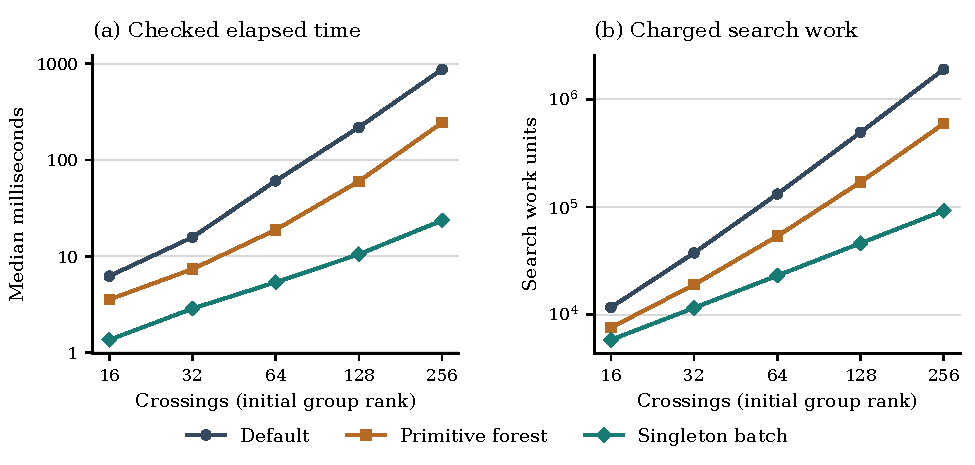
\includegraphics[width=\linewidth]{figures/stage_scaling.pdf}
\caption{Measured group-stage elapsed time and charged search work on the
same sources. Points are observed values; connecting segments aid reading
and are not fitted asymptotic laws. Earlier diagram simplification is
bypassed. The mathematical operation-count separation is proved separately.}
\label{fig:stage-scaling}
\end{figure}

At $n=256$, the median elapsed times are 876.7 ms for default, 244.6 ms for
forest, and 23.58 ms for singleton. The paired median improvements are
36.47 and 9.44, respectively. The large change is consistent with replacing
127 forest batches and 127 normalization handoffs by one batch containing
255 pivots. The corresponding work counters are 1,905,056, 595,473, and
92,547.

\begin{table}[tbp]
\centering
% Generated by experiments/summarize_singleton_dag.py; do not hand edit.
% One singleton batch in every row; nodes are search-arena total nodes.
\begingroup
\small\setlength{\tabcolsep}{4pt}
\begin{tabular}{rrrrrr}
\toprule
$n$ & Forest batches & Singleton pivots & Default nodes & Forest nodes & Singleton nodes \\
\midrule
16 & 7 & 15 & 419 & 121 & 147 \\
32 & 15 & 31 & 1611 & 249 & 307 \\
64 & 31 & 63 & 6299 & 505 & 627 \\
128 & 63 & 127 & 24891 & 1017 & 1267 \\
256 & 127 & 255 & 98939 & 2041 & 2547 \\
\bottomrule
\end{tabular}
\endgroup

\caption{Structural counters for the stage experiment. Every singleton
row uses one batch. Node counts are total allocated search-arena nodes,
including persistent nodes, rather than only reachable output nodes.}
\label{tab:stage-structure}
\end{table}

Singleton does not minimize every size measure. At 256 crossings the
forest arena has 2,041 nodes, while singleton has 2,547. The default has
98,939. The canonical JSON certificates occupy 49,244 bytes for forest,
12,770 for singleton, and 17,600 for default. The observed improvement
comes from avoiding repeated passes and normalization, not from a claim
that its arena is always smaller than the forest arena. The explicit
linear node formulas on this family and the general upper bound have
different meanings from finite elapsed times.

Across the stage cases, the paired A/A median ratios range from 0.901 to
1.104. This is enough variation to discourage fine interpretation of
small differences, while being far smaller than the large stage ratios
at the upper sizes. No speedup for the complete recognizer on this easy
family is inferred: an earlier simplifier can already close it.

\subsection{Ordinary whole-recognizer workload}

The ordinary experiment preserves all 19 cases and their original source
diagrams. It performs 570 measured calls and 114 excluded warmups, all of
which complete. The options include the group stage and relator operations,
compressed search, a group work allowance of 20,000,000, a group time
allowance of 10 seconds, an overall allowance of 12 seconds, and 50,000
objects. No incomplete call is silently dropped from a ratio.

Fifteen unknots reach the checked group stage. The trefoil and figure-eight
finish earlier through the homogeneous Seifert-genus filter; Conway and
Kinoshita--Terasaka finish through the modular Jones filter. Differences in
the times of these four early-closing knots cannot be attributed to a
singleton operation that was never reached.

\begin{table}[tbp]
\centering
% Generated by experiments/summarize_singleton_dag.py; do not hand edit.
% U_G: unknot via group stage; K_S: knotted via homogeneous Seifert genus; K_J: knotted via Jones. Only Gordian has a singleton batch.
\begingroup
\small\setlength{\tabcolsep}{4pt}
\begin{tabular}{llrrrr}
\toprule
Input & Outcome & Default ms & Forest ms & Singleton ms & Default/singleton \\
\midrule
survivor-00 & $\mathrm{U}_{G}$ & 12.022 & 13.303 & 11.997 & 0.970 \\
survivor-01 & $\mathrm{U}_{G}$ & 11.000 & 10.582 & 10.389 & 1.059 \\
survivor-02 & $\mathrm{U}_{G}$ & 12.929 & 11.724 & 11.987 & 0.943 \\
survivor-03 & $\mathrm{U}_{G}$ & 8.406 & 9.513 & 8.876 & 0.848 \\
mirror-03 & $\mathrm{U}_{G}$ & 23.508 & 24.634 & 18.523 & 1.245 \\
survivor-04 & $\mathrm{U}_{G}$ & 7.378 & 8.019 & 7.540 & 0.911 \\
survivor-05 & $\mathrm{U}_{G}$ & 18.598 & 19.196 & 15.077 & 1.234 \\
survivor-06 & $\mathrm{U}_{G}$ & 7.467 & 7.769 & 8.048 & 0.925 \\
survivor-07 & $\mathrm{U}_{G}$ & 14.327 & 15.372 & 20.256 & 0.747 \\
survivor-08 & $\mathrm{U}_{G}$ & 4.836 & 7.888 & 5.384 & 0.956 \\
mirror-08 & $\mathrm{U}_{G}$ & 13.089 & 14.260 & 15.950 & 0.807 \\
survivor-09 & $\mathrm{U}_{G}$ & 5.324 & 5.786 & 7.994 & 0.669 \\
survivor-10 & $\mathrm{U}_{G}$ & 4.759 & 4.740 & 5.076 & 0.889 \\
survivor-11 & $\mathrm{U}_{G}$ & 4.995 & 5.103 & 5.676 & 0.879 \\
gordian & $\mathrm{U}_{G}$ & 952.834 & 993.982 & 1005.899 & 0.950 \\
trefoil & $\mathrm{K}_{S}$ & 0.039 & 0.059 & 0.049 & 0.779 \\
figure-eight & $\mathrm{K}_{S}$ & 0.042 & 0.041 & 0.047 & 0.880 \\
conway & $\mathrm{K}_{J}$ & 0.637 & 0.622 & 0.655 & 0.952 \\
Kinoshita--Terasaka & $\mathrm{K}_{J}$ & 0.589 & 0.632 & 0.672 & 0.919 \\
\bottomrule
\end{tabular}
\endgroup

\caption{Completed whole-recognizer calls on the preserved ordinary corpus.
$\mathrm U_G$ means an unknot closed through the group stage;
$\mathrm K_S$ and $\mathrm K_J$ are knots closed by the Seifert-genus and
Jones filters. Times are median milliseconds, and the final column is the
paired median ratio. Only Gordian actually uses a singleton batch.}
\label{tab:ordinary}
\end{table}

Under the terminal guard, only Gordian uses the new operation. The other
fourteen unknots keep the default version-five proof while paying for
eligibility planning. Their individual timing variations are not evidence
that singleton contraction accelerated their search. Per-case A/A medians
span 0.896--1.249, including the very short cases.

For each measured round, sum the elapsed times over the complete 19-case
workload before forming a ratio. The medians of those five paired workload
ratios are
\[
 \frac{T_{\rm default}}{T_{\rm singleton}}=0.954856,
 \qquad
 \frac{T_{\rm forest}}{T_{\rm singleton}}=0.985518.
\]
Both favor the predecessor, with a modest overall difference. The analogous
workload A/A medians are 0.977439 for default, 0.986358 for forest, and
1.001674 for singleton. This is a workload-weighted aggregate, not a
typical-case estimate: Gordian accounts for about 86\% of total elapsed
time in each policy. Its medians
are 952.8, 994.0, and 1,005.9 ms in the same order. This record supports
keeping the feature opt-in and improving the cost of eligibility discovery.
It provides no ordinary-corpus acceleration or expanded recognition coverage.

\subsection{The failed eager policy and the delivered guard}

The earlier eager implementation applied a discovered batch whenever it
contained at least two pivots, even when many generators remained. Its
81-source audit yielded 53 positive certificates, no new positive, and
one lost positive: the 141-crossing Gordian fixture. The initial partial
batch eliminated 60 generators. Subsequent search on the changed residual
presentation exhausted the work allowance of 20,000,000 without producing
a certificate. The complete eager snapshot and audit are retained, so
the correction can be assessed against the actual counterexample.

The final guarded search skips 125 partial candidates on Gordian and later
uses a terminal batch of three pivots. Its version-eight certificate is
9,621 bytes. Its search work is 1,292,253, compared with 1,215,145 and a
9,663-byte proof for predecessor default. Thus the guard restores the
source-checked result in this experiment while adding some work. The 60
eager attempted pivots are reported as an unsuccessful experiment, not
added to the count of certified pivots.

The issue was downstream search behavior, not a failure of the exact
quotient theorem. The example makes a useful methodological point for
future work: a locally cheaper and algebraically sound transformation
can worsen a bounded heuristic. Productive exposure, residual-state
quality, and resource-aware scheduling need evidence and bounds of their
own. The terminal guard is a narrowly justified way to use the proved
operation while that research remains open.
